
Let us assume a knowledge graph using RDF with the introduced Turtle serialization as in listing \ref{lst:brackground_example_turtle_serialization}. However, over time, the knowledge graph has grown to have thousands of triples, and one would like to know the names of female persons who had contact with persons allergic to broccoli. This scenario is a simple example of the information needed, which can be expressed as a machine-interpretable query formulated in SPARQL. 
SPARQL -- short for SPARQL Protocol and Query Language -- is the W3C recommended declarative query language to query data from RDF graphs \cite{prudhommeaux2008sparql}. 

This section aims to provide the basic knowledge about SPARQL and the involved SPARQL set algebra used, such that the upcoming extension in section \ref{section_valSPARQL} can be clearly defined, and the reader can understand the basic types of queries used in this work. The notation defined here is mainly taken from Pérez et al. \cite{perez2009semantics} if not otherwise specified.

There are four different types of SPARQL queries called \uri{SELECT}, \uri{CONSTRUCT}, \uri{DESCRIBE} and \uri{ASK}. All query types use graph matching to identify which kind of data the author of the query is interested in. A query can be decomposed into a head and a body. While the head defines the query type containing its parameters and, therefore, defines the structure of the output, the body includes a graph pattern expression. 

Here the procedure is again done in a bottom-up fashion and, therefore, starts with defining the components used in graph pattern expressions. The atomic and pairwise distinct components are IRIs, blank nodes, literals, and variables. Three of them are already defined — the one left is the variables, which are referred to in the head of the query as parameters. 

\begin{Def}{Query Variables \cite{prudhommeaux2008sparql}}{sparql_variable}
A query variable is a Unicode string without spaces and prefixed with ``?''.
The infinite set of all possible query variables is denoted by $\mathbf{V}$ and is defined to be distinct with $\mathbf{I} \cup \mathbf{L} \cup \mathbf{B}$.
\end{Def}

Generally, a variable will be used in a graph pattern as a placeholder. When the graph pattern is evaluated over a knowledge graph, multiple solution mappings might exist. Each solution mapping assigns the variables the values that need to be substituted for the variables in the graph pattern in order for the graph pattern to match a subgraph of the knowledge graph. The value to be substituted can therefore be an IRI, a literal, or a blank node.

The graph pattern will be defined recursively, and the basic building block is always a triple pattern.

\begin{Def}{Triple Pattern \cite{prudhommeaux2008sparql}}{sparql_triple_pattern}
A triple pattern is a 3-tuple such that the infinite set of triple patterns $\mathbf{T}$ is a subset of $(\mathbf{I} \cup \mathbf{B} \cup \mathbf{V}) \times  (\mathbf{I} \cup \mathbf{V}) \times (\mathbf{I} \cup \mathbf{L} \cup \mathbf{B} \cup \mathbf{V})$. Additional the function $var: \mathbf{T} \to \mathcal{P}(\mathbf{V})$ is defined such that $\text{var}(t)$ gives the set of variables occurring in $t \in \mathbf{T}$. 
\end{Def}

Therefore, a triple pattern can be seen as an extended version of an RDF triple, allowing a variable in each position. At this point, it is helpful to have an idea of what a graph pattern will be. The following example is intended to give this intuition.

\begin{Bsp}{Visualization of a simple graph pattern}{graph_pattern_viz}
Let us return to the example query mentioned above, which should return the names of the female persons who had contact with persons allergic to broccoli. Analyzing the query gives three variables. The first one will be assigned a node referring to a female person, the second one to a node of the person allergic to broccoli, and the last will refer to the literal, which is the name of the female person. The query only asks for the name, but the other variables are still needed to define the graph pattern. 
The conjunction of six triple patterns is used to connect the variables. Though the conjunction is not yet defined, it will still make intuitive sense.
Figure \ref{fig:example_graph_pattern} shows the graph pattern visually using the notation explained in section \ref{background_rdf} with the addition of variables. This makes sense because a conjunction of triple patterns is just a set of RDF triples, which allows having variables in each position. A node representing a variable is of a diamond form. If it is a variable that will be returned finally, the node is double lined. 

Evaluating the graph pattern against the knowledge graph in figure \ref{fig:example_graph_pattern_evaluation} will give a set of solution mappings. In this example the set consists of one solution mapping of ?name to ``Maria''. Figure \ref{fig:example_graph_pattern_evaluation} additionally depicts the evaluation by highlighting the subgraph, matched by the graph pattern from figure \ref{fig:example_graph_pattern}, used to produce a solution mapping. 
\captionsetup{type=htypei}
    \begin{minipage}[t]{\linewidth}
            \centering
            \vspace{1ex}
            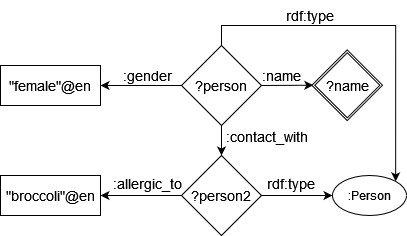
\includegraphics[width=7cm]{images/sparql/graph_pattern_viz.png}
            \captionof{figure}{An Example Graph Pattern. It will query the names of female persons, which had contact to persons allergic to broccoli}
            \label{fig:example_graph_pattern}
            \vspace{1ex}
        \end{minipage}
 
\captionsetup{type=htypei}
    \begin{minipage}[t]{\linewidth}
            \centering
            \vspace{1ex}
            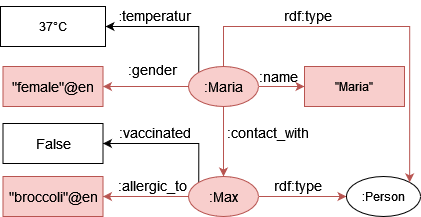
\includegraphics[width=7cm]{images/sparql/graph_pattern_viz_kg.png}
            \captionof{figure}{A small Knowledge Graph. The red subgraph is matched by the graph pattern from figure \ref{fig:example_graph_pattern} to produce a solution mapping.}
            \label{fig:example_graph_pattern_evaluation}
    \end{minipage}
\end{Bsp}

As in the example, evaluating a graph pattern expression $P$ over a knowledge graph $G$ gives a set of solution mappings. Each solution mapping maps at least the variables used outside of an \uri{OPTIONAL} pattern to RDF terms. The \uri{OPTIONAL} pattern will be defined together with the graph pattern expression in definition \ref{Def:sparql_graph_pattern}. A single solution mapping is defined as follows.

\begin{Def}{SPARQL Solution Mapping \cite{prudhommeaux2008sparql}}{sparql_solution_mapping}
A solution mapping is a partial function $\mu: \mathbf{V} \to (\mathbf{B} \cup \mathbf{L} \cup \mathbf{I})$, which maps a subset of the infinite set of variables $\mathbf{V}$ to RDF terms. %The variables, which got a RDF term assigned by $\mu$, can be retrieved with $\text{dom}(\mu)$.
Two mappings $\mu_1$ and $\mu_2$ are called compatible, denoted with $\mu_1 \sim \mu_2$, when $\forall v \in (\text{dom}(\mu_1) \cap \text{dom}(\mu_1)) ~ \mu_1(v) = \mu_2(v)$ is true. In that case the union of two mappings $\mu_1$ and $\mu_2$ is defined as $\mu_1 \cup \mu_2$, which is a shorthand for $\mathcal{G}_{\mu_1} \cup \mathcal{G}_{\mu_2}$.
The infinite set of all possible SPARQL solution mappings is defined to be $\mathbf{M}$.
\end{Def}

Next, algebraic operations over the sets of solution mappings and filter conditions on a set of solution mappings are needed to recursively extend the notion of the graph pattern with further operators.
A filter condition is a logical expression $R \in \mathcal{L_\mathbb{S}}$ with $\mathbb{S} = (\mathbf{B} \cup \mathbf{L} \cup \mathbf{I}; {<}; {+,*};{0,1})$, which makes use of variables from $\mathbf{V}$. There are further functions defined and, moreover, the functions and relations in the structure can only be applied to specific types of literals. IRIs can only be checked for equality as there is no order defined. All this is specified exactly in \cite{prudhommeaux2008sparql}.
Nevertheless, a filter condition $R$ can be evaluated via $(\mathbb{S}, \mu) \models R$ using the solution mapping $\mu$ as an assignment.

The algebraic operations over sets of solution mappings are the content of the following definition.

\begin{Def}{Algebraic Operations over sets of solution mappings (extended version of \cite{schmidt2010foundations})}{algebra_solution_mapping}
Given two sets of solution mappings $\Omega_1, \Omega_2 \subset \mathbf{M}$, a set of variables $v \subset \mathbf{V}$, a filter condition $R \in \mathcal{L_\mathbb{S}}$ and a function used for renaming of variables $\mathcal{r}:\mathbf{V} \to \mathbf{V}$ the following operations are defined:
\begin{center}
            \begin{tabular}{l|l}
             \toprule
             operation & meaning \\
             \midrule
             \midrule
             $\pi_v(\Omega_1)$ & $\{\mu_1 \mid \exists \mu_2 : \mu_1 \cup \mu_2 \in \Omega_1 \land \text{dom}(\mu_1) \subseteq v \land (\text{dom}(\mu_2) \cap v) = \emptyset \}$ \\
             $\sigma_R(\Omega_1)$ & $\{\mu \in \Omega_1 \mid (\mathbb{S}, \mu) \models R \}$ \\
             $\Omega_1 \cup \Omega_2$ & $\{\mu \mid \mu \in \Omega_1 \lor \mu \in \Omega_2 \}$ \\
             $\Omega_1 \bowtie \Omega_2$ & $\{\mu_1 \cup \mu_2 \mid \mu_1 \in \Omega_1, \mu_2 \in \Omega_2 : \mu_1 \sim \mu_2\}$ \\
             $\Omega_1 \setminus \Omega_2$ & $\{\mu_1 \in \Omega_1 \mid \forall \mu_2 \in \Omega_2 : \neg (\mu_1 \sim \mu_2)\}$ \\
             $\rho(\mathcal{r},\Omega_1)$ & $\{ \mathcal{r} \circ \mu \mid \mu \in \Omega_1\}$\\
             \bottomrule
        \end{tabular}
\end{center}
Compared to Schmidt et al., $\rho$ is added to the algebraic operations to allow for variable renamings in solution mappings. $\mathbb{S}$ is the structure $(\mathbf{B} \cup \mathbf{L} \cup \mathbf{I}; {<}; {+,*};{0,1})$
\end{Def}

Before the notion of a graph pattern and its evaluation can be appropriately defined, there is the substitution of a solution mapping into the triple pattern left. A thing which was already implicitly done in example \ref{Bsp:graph_pattern_viz} to identify the red subgraph.
To do that formally, $\mu$ is overloaded to be usable as a function $\mu: \mathbf{T} \to (\mathbf{I} \cup \mathbf{B}) \times \mathbf{I} \times (\mathbf{I} \cup \mathbf{L} \cup \mathbf{B})$, such that $\mu(t)$ replaces all occurrences of $v \in \text{dom}(\mu)$ in $t$ with $\mu(v)$. 

Now the graph pattern expression and their evaluation can be formally defined:

\begin{Def}{Graph Pattern Expression and their Evaluation (similar to \cite{perez2009semantics, schmidt2010foundations})}{sparql_graph_pattern}
Let $t\in \mathbf{T}$ be a triple pattern as defined in definition \ref{Def:sparql_triple_pattern}. The following table gives the recursive definition of a graph pattern $P$, the SPARQL syntax and the evaluation of the graph pattern into the set of solution mappings. The infinite set of all graph patterns is denoted as $\mathbf{P}$. The evaluation of a graph pattern $P \in \mathbf{P}$ over the knowledge graph $G \in \mathbf{G}$ is written as a function $[[P]]_G: \mathbf{P} \times \mathbf{G} \to \mathcal{P}(\mathbf{M})$ and gives a set of SPARQL mappings as defined in definition \ref{Def:sparql_solution_mapping}.  The recursive definition of a graph pattern assumes that $P_1$, $P_2$ are graph patterns, $R$ is a filter condition, $v \subset \mathbf{V}$ and $\mathcal{r}$ a renaming function as in definition \ref{Def:algebra_solution_mapping}.
\begin{center}
            \begin{tabular}{l|l|l}
             \toprule
             graph pattern $P$ & syntax & evaluation $[[P]]_G$ \\
             \midrule
             \midrule
             $t := (s,p,o)$ & $s$ $p$ $o$ & $\{\mu \mid \text{dom}(\mu) = var(t) \land \mu(t) \in E_G\}$\\
             $(P_1 \text{\uri{ AND }} P_2)$ & $\{P_1 \text{\uri{ . }} P_2\}$ &  $[[P_1]]_G \bowtie [[P_2]]_G$ \\
             $(P_1 \text{\uri{ UNION }} P_2)$ & $\{\{P_1\}\text{\uri{ UNION }}\{P_2\}\}$ & $[[P_1]]_G \cup [[P_2]]_G$\\
             $(P_1 \text{\uri{ OPT }} P_2)$ & $\{\{P_1\}\text{\uri{ OPTIONAL }}\{P_2\}\}$ & $[[P_1]]_G \leftouterjoin [[P_2]]_G$\\
             $(P_1 \text{\uri{ FILTER }} R)$ &  $\{\{P_1\}\text{\uri{ FILTER }} R\}$ & $\sigma_R([[P_1]]_G)$\\
             $\text{\uri{SELECT}}(v, \mathcal{r}, P_1)$ & $\{\text{\uri{SELECT }} v' \text{\uri{ WHERE }} \{P_1\}\}$ & $\rho(\mathcal{r}, \pi_v([[P_1]]_G)$\\
             \bottomrule
        \end{tabular}
\end{center}
$v'$ denotes $v$ but written as a list separated with spaces. Additionally, there is the option to implicitly define $\mathcal{r}$ with the \uri{AS} keyword used in-place between the renamed variable $\text{var} \in v$ and the new variable $\text{new} \in \mathbf{V}$. All other variables not included on the left-hand side of the \uri{AS} keyword will be mapped to themself.
\end{Def}

Turtle is used for serializing the graph patterns in $\mathbf{P}$. Therefore, serializing a graph pattern is just a matter of serializing the triple patterns with Turtle and writing down the other operators using the syntax as defined. For example, a conjunction (``\uri{AND}'') of triple patterns is denoted with a dot. The other short hands presented as Turtle's features to shorten the conjunctions of RDF triples can also be used. There are further rules of precedence, association, syntax, and operators (like the concept of grouping) defined in SPARQL, which abstract away from the logical core. These allow to relax the requirements for the brackets in definition \ref{Def:sparql_graph_pattern} and can be found in \cite{prudhommeaux2008sparql}. 

Now that the basic syntax of the body of a SPARQL query is defined by serializing graph patterns, one has to define the head. In this work, only \uri{SELECT} queries are used, such that it will be enough to define this query type.

\begin{Def}{SPARQL \uri{SELECT} Query}{sparql_query}
A SPARQL \uri{SELECT} query $Q$ is a graph pattern $P$ of the form $\text{\uri{SELECT}}(var(Q), \mathcal{r},P')$ where $P' \in \mathbf{P}$ and $\mathcal{r}$ a renaming function as defined in \ref{Def:algebra_solution_mapping}. $P$ uses the syntax as defined for the \text{\uri{SELECT}} clause in definition \ref{Def:sparql_graph_pattern} but without the outermost brackets. The infinite set of SPARQL \uri{SELECT} queries is denoted with $\mathbf{Q}$.
\end{Def}

Like Turtle, SPARQL allows the definition of prefixes but instead of ``\uri{@prefix}'', \glqq\uri{PREFIX}'' is used.
To show the algebra and the SPARQL syntax in action, the following example continues example \ref{Bsp:graph_pattern_viz}.

\begin{Bsp}{SPARQL Algebra and syntax applied}{sparql_algreba_syntax}
Given the visualization, in example \ref{Bsp:graph_pattern_viz} the triple patterns lying at the heart of the graph pattern and needed to specify the query can be identified. All of the triple patterns should apply simultaneously, implying the need for the conjunction of the triple patterns. In the end, only the names of the persons should be retrieved, such that only ?name is projected. There is no renaming of variables needed here. Therefore, the identity function $\text{id}$ mapping each variable to itself is used.
\begin{align*}
        \text{\uri{SELECT}(?name,$\text{id}$,} & \text{((((((?person, \uri{:gender}, ''female@en'')} \\
        &\text{\uri{ AND }} \text{(?person, \uri{rdf:type}, :Person))} \\
        &\text{\uri{ AND }} \text{(?person, \uri{:name}, ?name))} \\
        &\text{\uri{ AND }} \text{(?person, \uri{:contact\_with}, ?person2))} \\
        &\text{\uri{ AND }} \text{(?person2, \uri{:allergic\_to}, ''broccoli''@en))} \\
        &\text{\uri{ AND }} \text{(?person2, \uri{rdf:type}, :Person)))} \\
\end{align*}
Using the left associative property of \text{\uri{AND}}, the algebra can be transformed into the SPARQL syntax.

    \lstset{language=html}
    \begin{lstlisting}[captionpos=b, caption=Algebra transformed into SPARQL syntax , label=lst:sparql_algebra_example, basicstyle=\ttfamily, frame=single]
    PREFIX : <http://example.org/>
    SELECT ?name WHERE {
        ?person :gender ''female''@en .
        ?person a :Person
        ?person :name ?name .
        ?person :contact_with ?person2 .
        ?person2 :allergic_to ''broccoli''@en .
        ?person2 a :Person
    }

    \end{lstlisting}
\end{Bsp}


Finally, given a SPARQL \uri{SELECT} query the evaluation of the query is defined analogue to the evaluation of a graph pattern.

\begin{Def}{Execution of $Q$ over $G$ \cite{corman2019validating}}{executing_q_over_g}
The execution of the SPARQL \uri{SELECT} query $Q \in \mathbf{Q}$ over the knowledge graph $G \in \mathbf{G}$ is written as a function $[[Q]]_G: \mathbf{Q} \times \mathbf{G} \to \mathcal{P}(\mathbf{M})$ and gives a set of SPARQL mappings. Each SPARQL mapping assigns the set of variables $var(Q) \subset \mathbf{V}$ to RDF terms.
\end{Def}

It is essential to note that a SPARQL endpoint typically performs the process of executing a query over a knowledge graph. The SPARQL endpoint exposes a knowledge graph by answering SPARQL queries using the knowledge graph. Most knowledge graphs are exclusively accessible using SPARQL queries, which consolidates the use of SPARQL as the primary medium to extract information from a knowledge graph.
